\documentclass[]{beamer}
\usepackage{graphicx} 
\graphicspath{{Images/}{./}}
\usepackage{booktabs}
\usepackage{tikz}
\usepackage{pgfplots}
\usepackage{float}
\usepackage{listings,xcolor}

\usetheme{Madrid}
\usecolortheme{beaver}
\usefonttheme{default} 
\usepackage{palatino}
\usepackage[default]{opensans}
\useinnertheme{default}
\usepackage[german]{babel}
\usepackage{caption}



\setbeamertemplate{footline}{}
\setbeamertemplate{navigation symbols}{}
\setbeamertemplate{headline}{}


\title[]{Zwischenpräsentation}

\author[shortname]{David Metzler \and Emircan Tutar  \and Niklas Kleiser}

\institute[shortinst]{ Hochschule Ravensburg Weingraten\\ \smallskip} 

\date{ \today}
%----------------------------------------------------------------------------------------

\begin{document}


%----------------------------------------------------------------------------------------
%	TITLE SLIDE
%----------------------------------------------------------------------------------------

\begin{frame}
	\titlepage % Output the title slide, automatically created using the text entered in the PRESENTATION INFORMATION block above
\end{frame}

%----------------------------------------------------------------------------------------
%	TABLE OF CONTENTS SLIDE
%----------------------------------------------------------------------------------------

% The table of contents outputs the sections and subsections that appear in your presentation, specified with the standard \section and \subsection commands. You may either display all sections and subsections on one slide with \tableofcontents, or display each section at a time on subsequent slides with \tableofcontents[pausesections]. The latter is useful if you want to step through each section and mention what you will discuss.

\begin{frame}
	\frametitle{Presentation Overview} % Slide title, remove this command for no title
	
	\tableofcontents % Output the table of contents (all sections on one slide)
	%\tableofcontents[pausesections] % Output the table of contents (break sections up across separate slides)
\end{frame}

%----------------------------------------------------------------------------------------
%	PRESENTATION BODY SLIDES
%----------------------------------------------------------------------------------------

\section{Systemaufbau}
\begin{frame}{Systemaufbau}

  \begin{figure}
    \begin{tikzpicture}[scale=0.76]
		
		\draw [-, dashed, gray] (4,1)-- (-4,1)--(-4,3.5) --(4,3.5) --(4,1);
		\node at (-2.8 ,3) {BED VIEW};
					
		\node[inner sep=0pt] (whitehead) at (2,2.5)
		{
\includegraphics[width=.05\textwidth]{Images/camera.png}};
		
		\node[above] at (2.2,2.6) {\scriptsize Raspberry Pi};
		
		\node[inner sep=0pt] (whitehead) at (0,2)
		{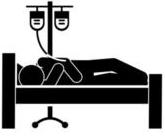
\includegraphics[width=.1\textwidth]{Images/person_in_bed.png}};

			\node at (-2.5 ,-1) {ROOM VIEW};
	
			\draw [-, dashed, gray] (4,-0.5)-- (-4,-0.5)--(-4,-4) --(4, -4 ) --(4,-0.5);
		
		\node[inner sep=0pt] (whitehead) at (2,-1.5)
		{
\includegraphics[width=.05\textwidth]{Images/camera.png}};
		

		
		\node[inner sep=0pt] (whitehead) at (-0.25,-1.25)
		{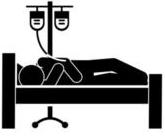
\includegraphics[width=.1\textwidth]{Images/person_in_bed.png}};
		
		
		\node[inner sep=0pt] (whitehead) at (0,-2.25)
		{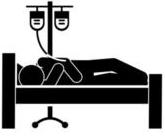
\includegraphics[width=.1\textwidth]{Images/person_in_bed.png}};
		
	\node[inner sep=0pt] (whitehead) at (-0.5,-3.25)
		{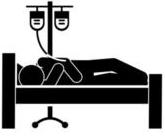
\includegraphics[width=.1\textwidth]{Images/person_in_bed.png}};
		

	  \node[inner sep=0pt] (whitehead) at (4.0,0.25)
		{
\includegraphics[width=.06\textwidth]{Images/server.png}};
		
				\node[below] at (2.2,-1.6) {\scriptsize Raspberry Pi};
		
		\node[below] at (4.0,0) {\scriptsize Broker};
		
			
		
		\draw [-] (2,2.5)-- ( 3,2.5) -- (3,0.25) ;
		\draw [-] (2,-1.5)-- ( 3,-1.5) -- (3,0.25) ;
		\draw [-]  (3,0.25)  -- (3.8,0.25);

	    \draw [->]  (4.2 ,0.25) -- (5.0,0.25) -- (5.0,-1.5) -- (5.5,-1.5);
	     \draw [->]  (4.2 ,0.25) -- (5.0,0.25) -- (5.0,2.5) -- (5.5,2.5);
	
		\node at  (7.0,2.5) {\scriptsize Bed Detection};
		
		
		\node at  (7.0,-1.5) {\scriptsize Fall Detection};
		
		
	
	 	\draw [->]  (8.5 ,-1.5) -- (9.0,-1.5) -- (9,0.25) -- (9.5,0.25)  ;
	
		\draw [->]  (8.5, 2.5) -- (9.0,2.5) -- (9,0.25) -- (9.5,0.25) ;
		
		\node[inner sep=0pt] (whitehead) at (9.85,0.25)
		{
\includegraphics[width=.05\textwidth]{Images/raspi.png}};
		
		\node[below] at (9.8,-0.1) {\scriptsize Pi };
		
		\draw [->]  (10.3,0.25) -- (10.6,0.25) ;
		
		\node[red] at  (11.4,0.25) {Alarm};
		
		
	\end{tikzpicture}
        \caption{Darstellung des Systemaufbaus}
	\label{fig:patient_monitoring}

  \end{figure}

    
\end{frame}

\section{Lastenheft}
\subsection{Muss - Anforderungen}
\begin{frame}
\frametitle{Lastenheft}
\framesubtitle{Muss - Anforderungen}
\begin{enumerate}
    \item Docker
    \item Ubuntu 22.04 (LTS)
    \item Dynamisches DNS-Management (ddclient)
    \item Fail2ban
    \item MQTT / MQTT-Client
    \item SMTP-Server / SMTP-Client
    \item Raspberry und Raspberry Pi
    \item Fall Detektion
    \item Matrix
\end{enumerate}
\end{frame}

\subsection{Soll - Anforderungen}
\begin{frame}
\frametitle{Lastenheft}
\framesubtitle{Soll - Anforderungen}
\begin{enumerate}
    \item Bett Detektion
    \item Alarm (Ton und Licht)
    \item Firewall
\end{enumerate}
\end{frame}

\subsection{Kann - Anforderungen}
\begin{frame}
\frametitle{Lastenheft}
\framesubtitle{Kann - Anforderungen}
\begin{enumerate}
    \item MQTT Frontend
    \item Gesprochene Information über Patient in Hilfesituation
    \item Kameraview
\end{enumerate}
\end{frame}



\section{Aktueller Stand}
\subsection{Setup Hardware}
\begin{frame}
\frametitle{Setup}
\framesubtitle{Hardware}
\begin{enumerate}
    \item 3 Raspberry Pi
    \item 1 Kamera ist da
    \item Ubuntu 22.04 installiert
\end{enumerate}
\end{frame}


\section{Aktueller Stand}
\subsection{Raspberry PI}
\begin{frame}
	\frametitle{Setup}
	\framesubtitle{Raspberry PI}
 \begin{figure}
	\centering
	\begin{minipage}[t]{0.45\textwidth} 
		\centering
		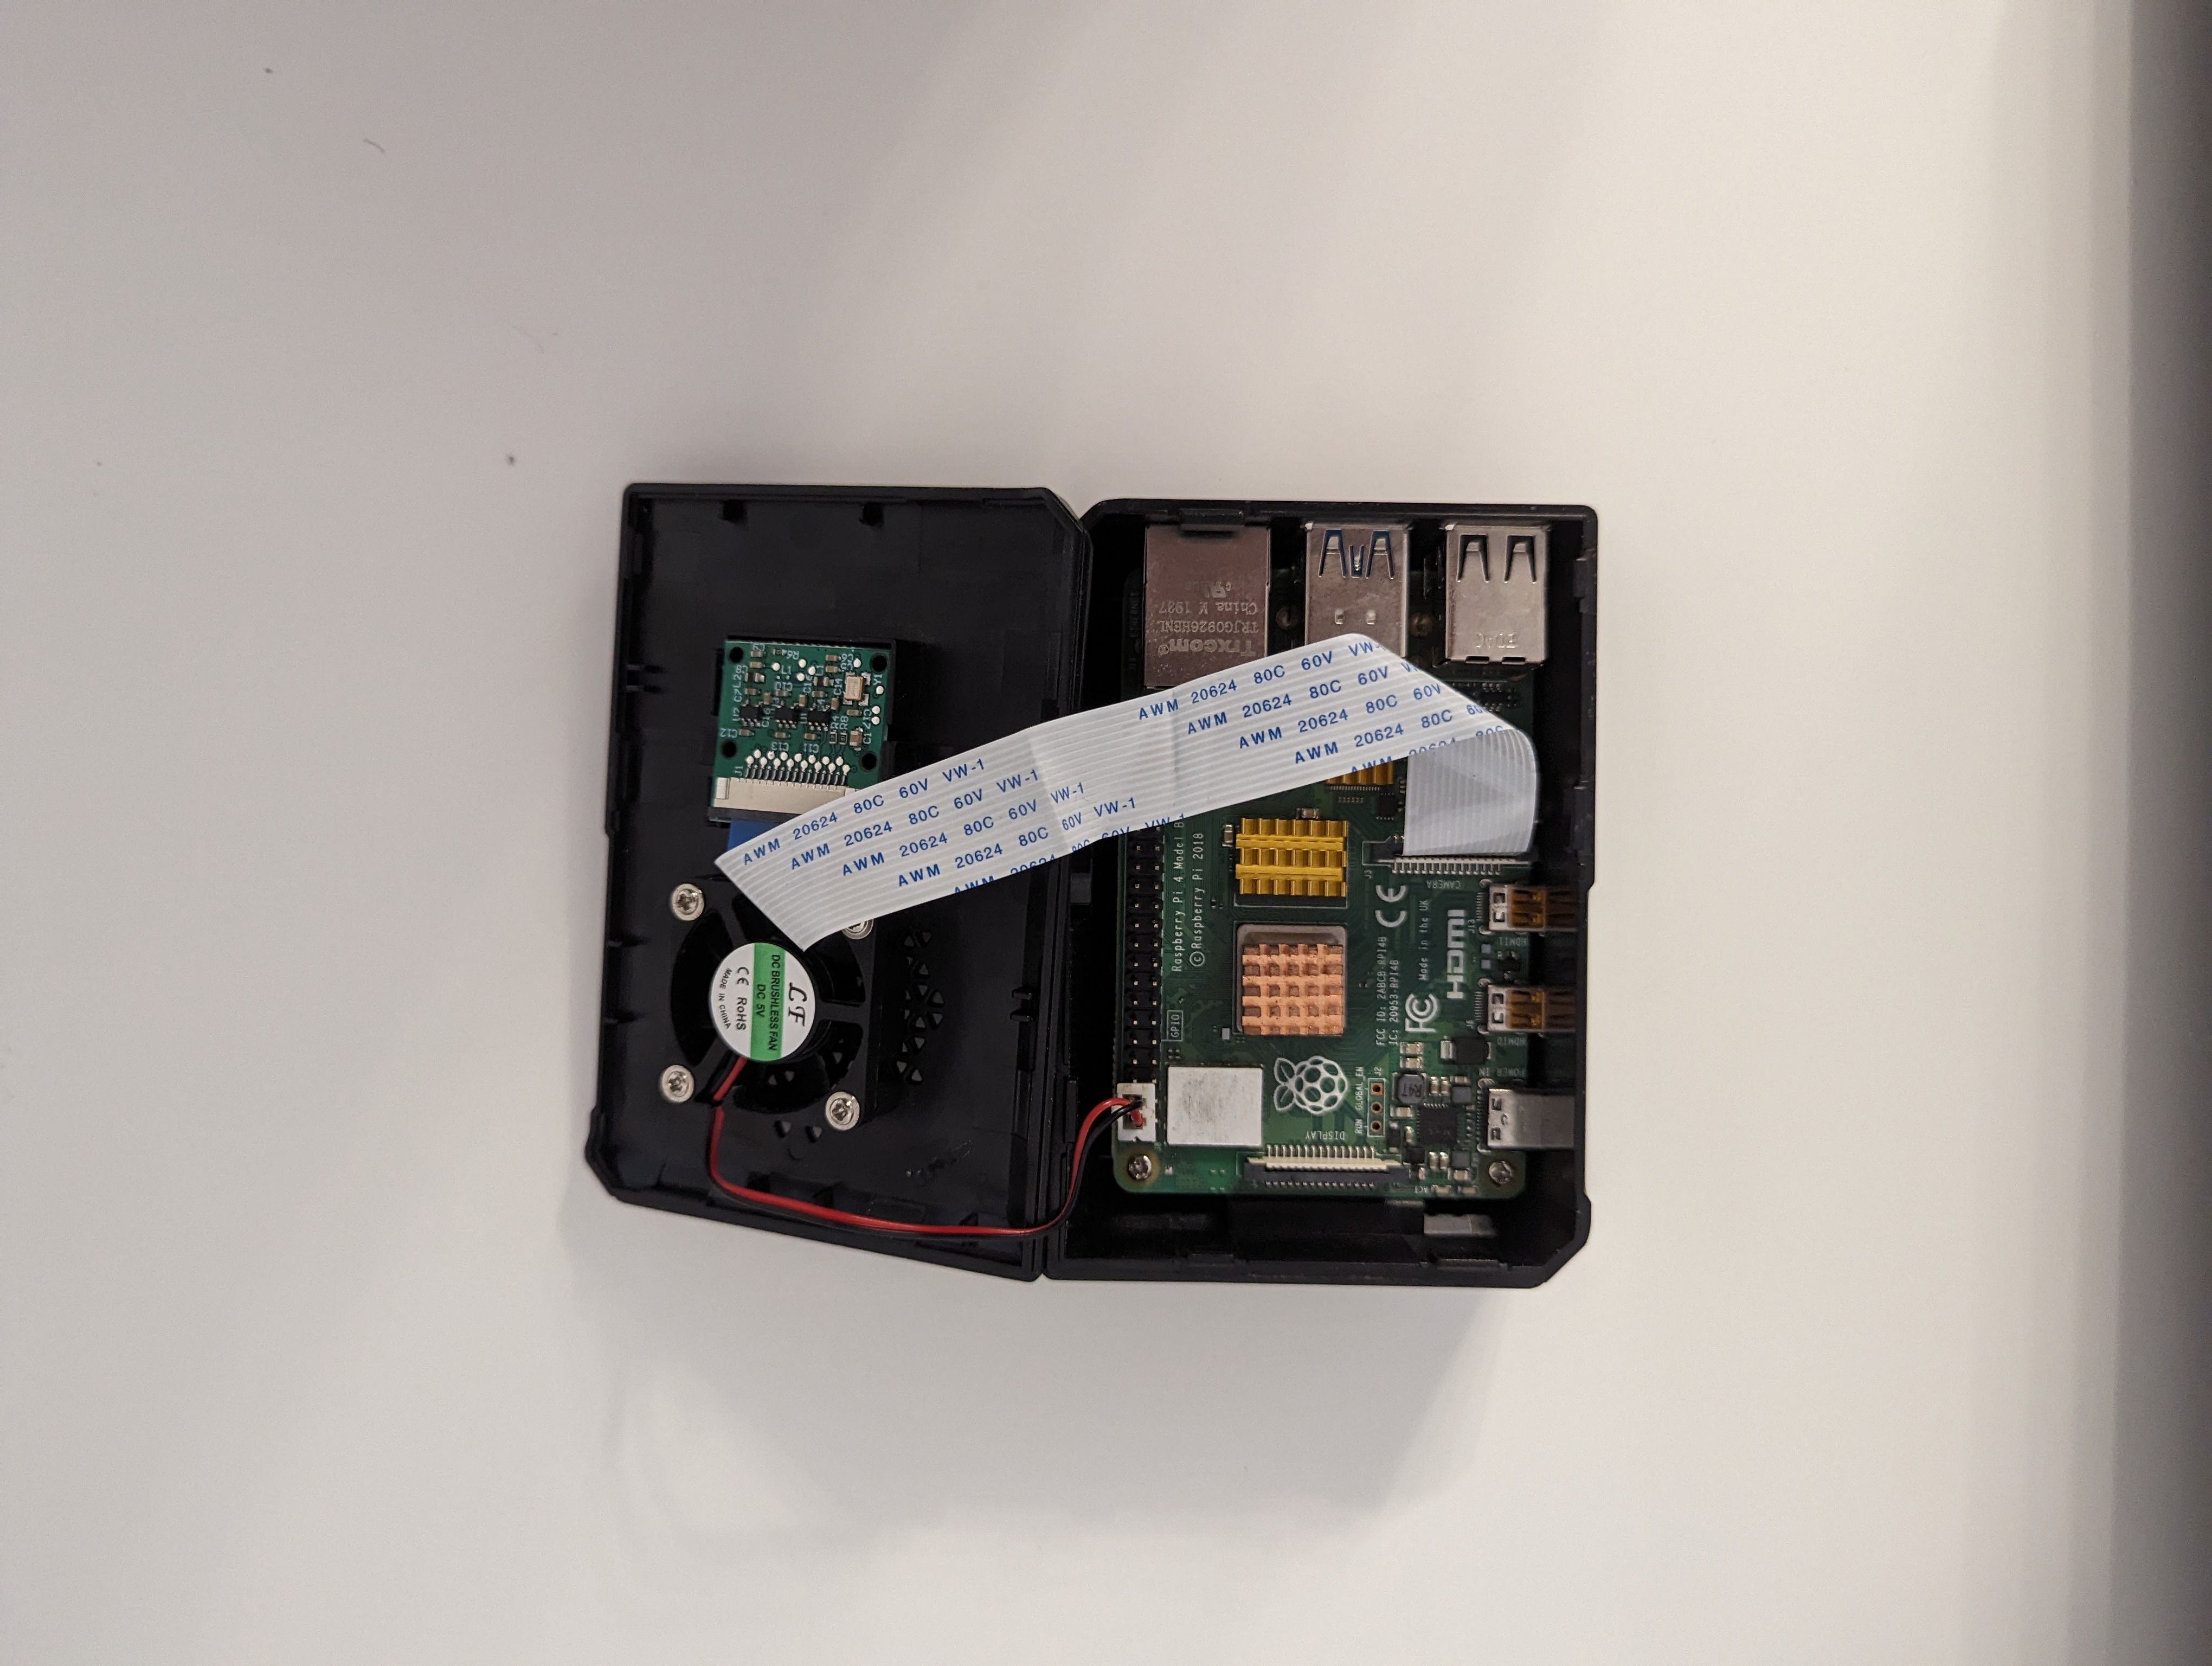
\includegraphics[width=0.8\textwidth]{Images/Raspberry_Pi_and_Camera_Open.jpg} 
		\caption*{Aufbau im Gehäuse}
	\end{minipage}
	\hfill
	\begin{minipage}[t]{0.45\textwidth} 
		\centering
		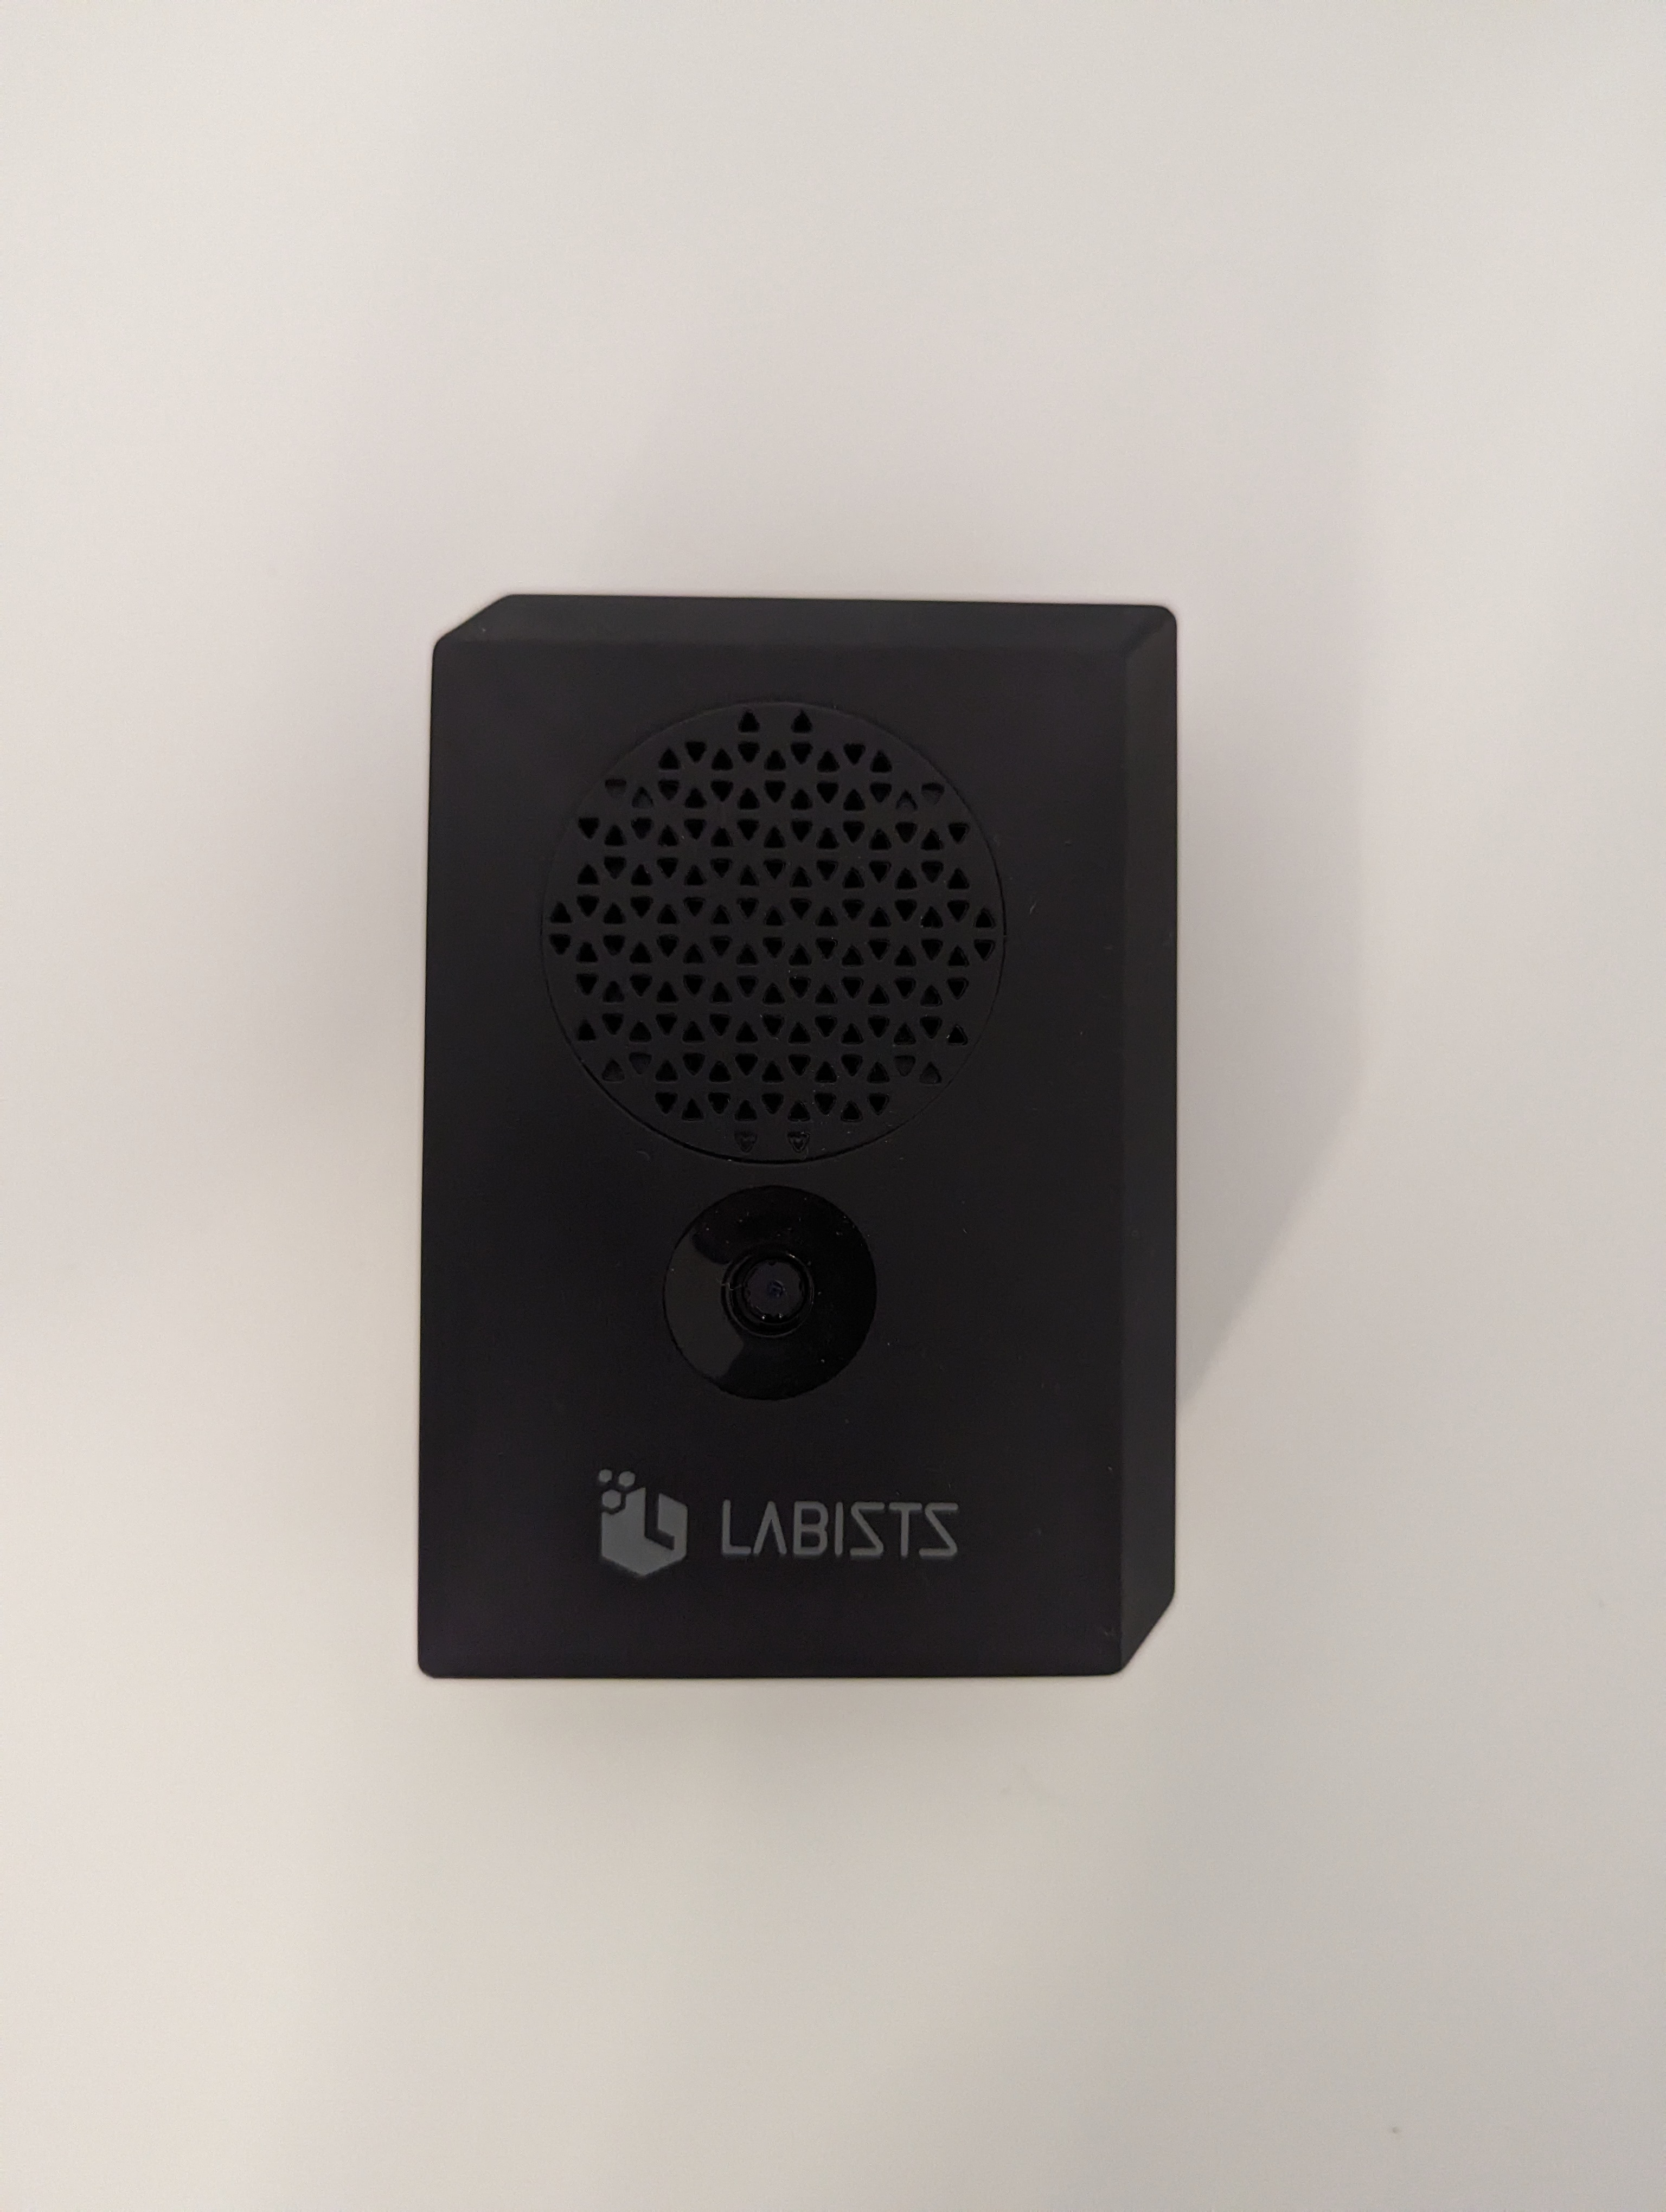
\includegraphics[width=0.6\textwidth]{Images/Raspberry_Pi_and_Camera_Closed.jpg}
		\caption*{Gehäuse mit Kamera}
	\end{minipage}
	\hfill
	\caption{Raspberry Pi mit Kamera}
	\label{fig:Raspberry PI}
\end{figure} 
\end{frame}



\subsection{Setup Software}
\begin{frame}
\frametitle{Setup}
\framesubtitle{Software}

\begin{enumerate}
    \item Docker und Docker Compose
    \item UFW
    \item DDClient (noch ohne Docker)
\end{enumerate}
\end{frame}

\subsection{Alarm}
\begin{frame}
\frametitle{Aktueller Stand}
\framesubtitle{Alarm}
\begin{enumerate}
    \item Steckboard und Pins bereit
    \item LEDs bereit
    \item Lautsprecher wird ausgeliehen
    \item 3.Rasberry Pi im Versand 
\end{enumerate}
\end{frame}


\subsection{MQTT}
\begin{frame}
\frametitle{Aktueller Stand}
\framesubtitle{MQTT}
\begin{enumerate}
    \item Konzept ausgearbeitet
    \item Erste Implementation \& Local - Deployment
    \item MR in Review
\end{enumerate}
\end{frame}


\subsection{YOLO}
\begin{frame}
\frametitle{Aktueller Stand}
\framesubtitle{YOLO}
\begin{enumerate}
    \item Pretrained Model für Anforderugnen gefunden 
    \item Container aufgesezt
    \item Inklusion in MQTT  fertig
\end{enumerate}

\end{frame}

\begin{frame}
\frametitle{Aktueller Stand}
\framesubtitle{YOLO}
\begin{figure}
	\centering
	\begin{minipage}[t]{0.3\textwidth}
		\centering
		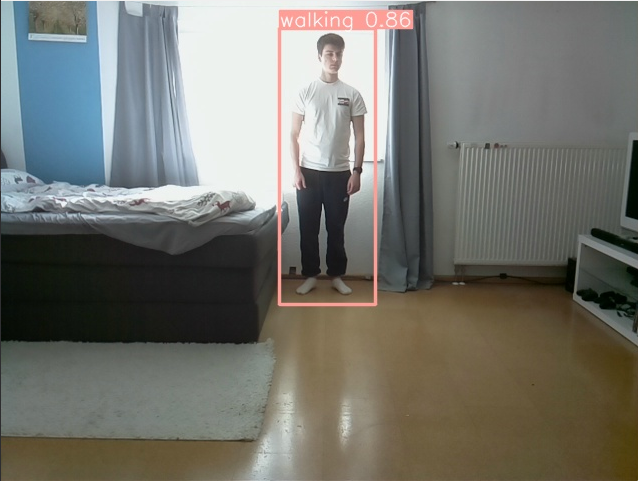
\includegraphics[width=\textwidth]{Images/walking.png}
		\caption*{''walking''}
	\end{minipage}
	\hfill
	\begin{minipage}[t]{0.3\textwidth}
		\centering
		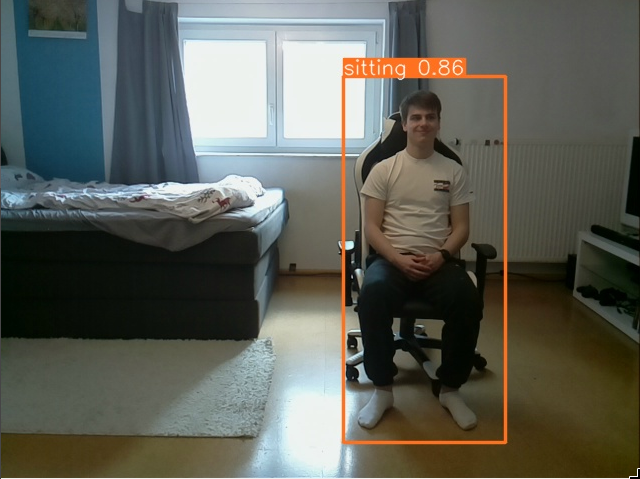
\includegraphics[width=\textwidth]{Images/sitting.png}
		\caption*{''sitting''}
	\end{minipage}
	\hfill
	\begin{minipage}[t]{0.3\textwidth}
		\centering
		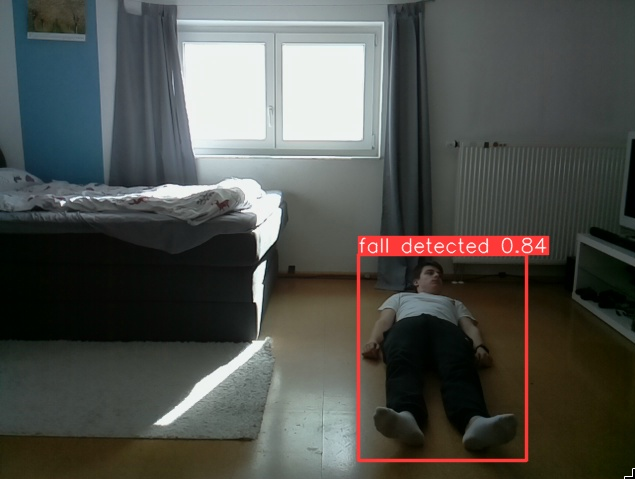
\includegraphics[width=\textwidth]{Images/fallen.png}
		\caption*{ ''fall detected''}
	\end{minipage}
	\caption{YOLOv5 Klassen}
	\label{fig:yolo_classes}
\end{figure}

\end{frame}


\subsection{Matrix}
\begin{frame}
\frametitle{Aktueller Stand}
\framesubtitle{Matrix}
\begin{enumerate}
    \item Matrix Server aufgesetzt
    \item E-Mail Bridge eingebunden
    \item Element als Client ausgewählt
\end{enumerate}
\end{frame}

\begin{frame}
	\frametitle{Aktueller Stand}
	\framesubtitle{Matrix}
 \begin{figure}
	\centering
	\begin{minipage}[t]{0.45\textwidth} 
		\centering
		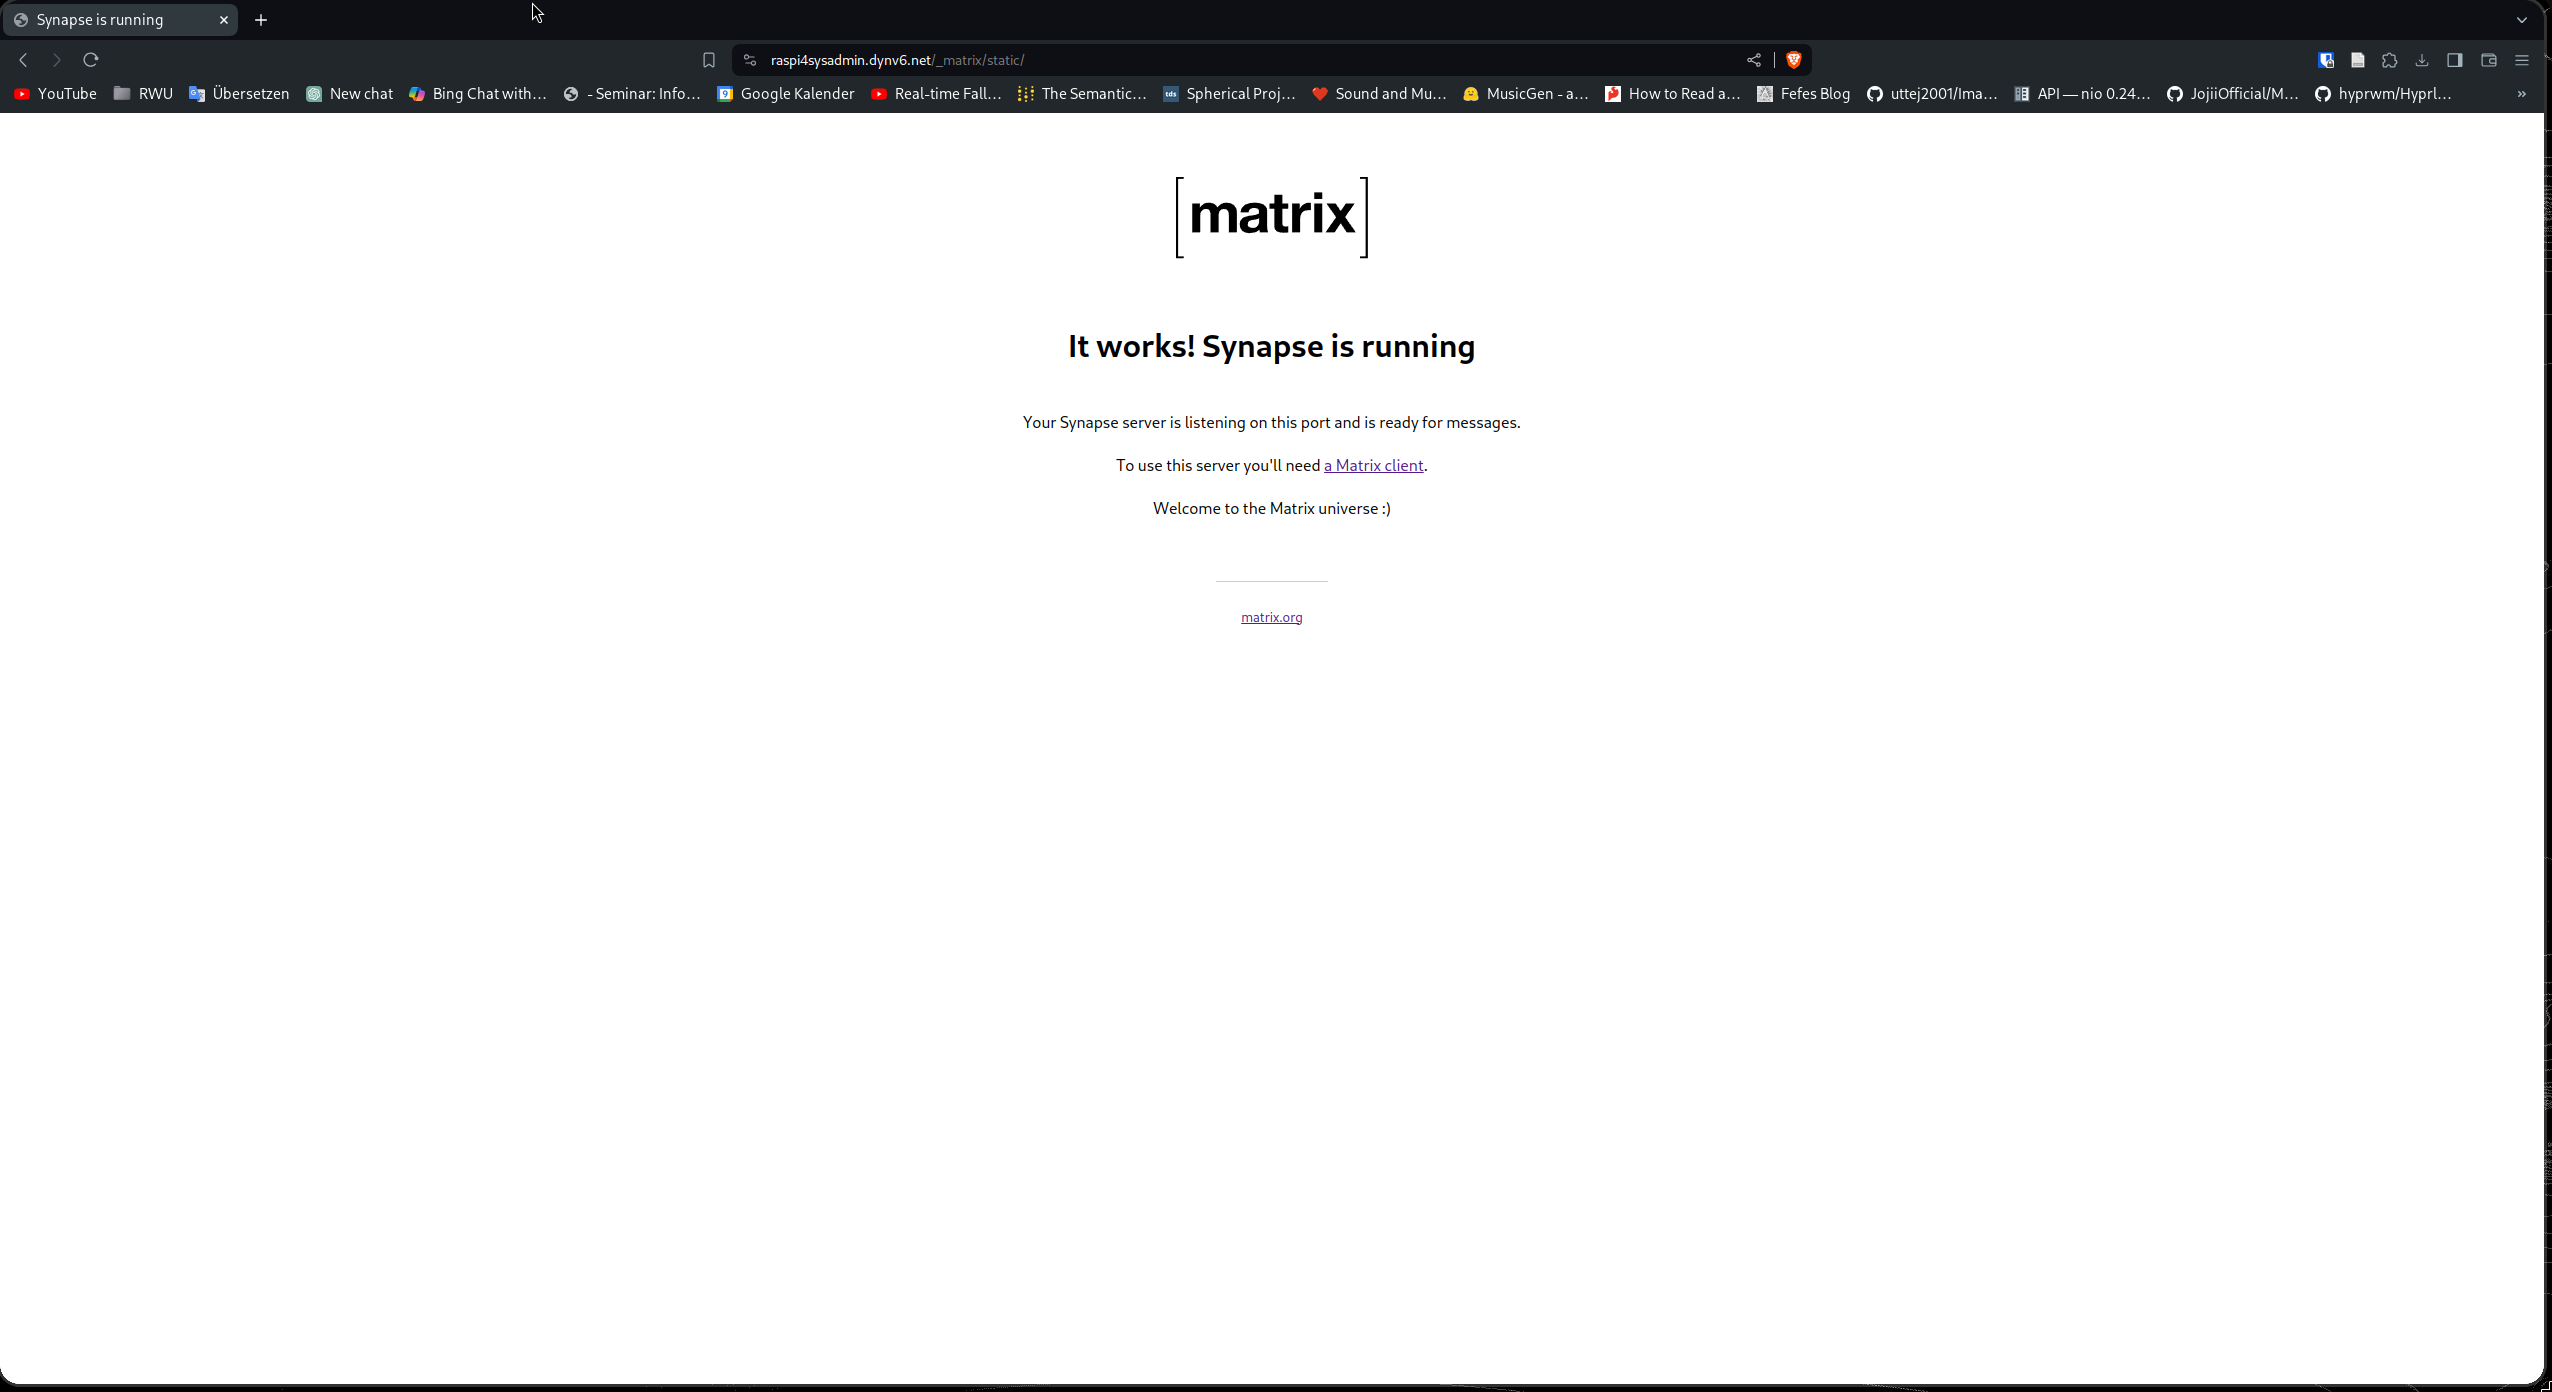
\includegraphics[width=\textwidth]{Images/Matrix_2.png} 
		\caption*{Matrix Server}
	\end{minipage}
	\hfill
	\begin{minipage}[t]{0.45\textwidth} 
		\centering
		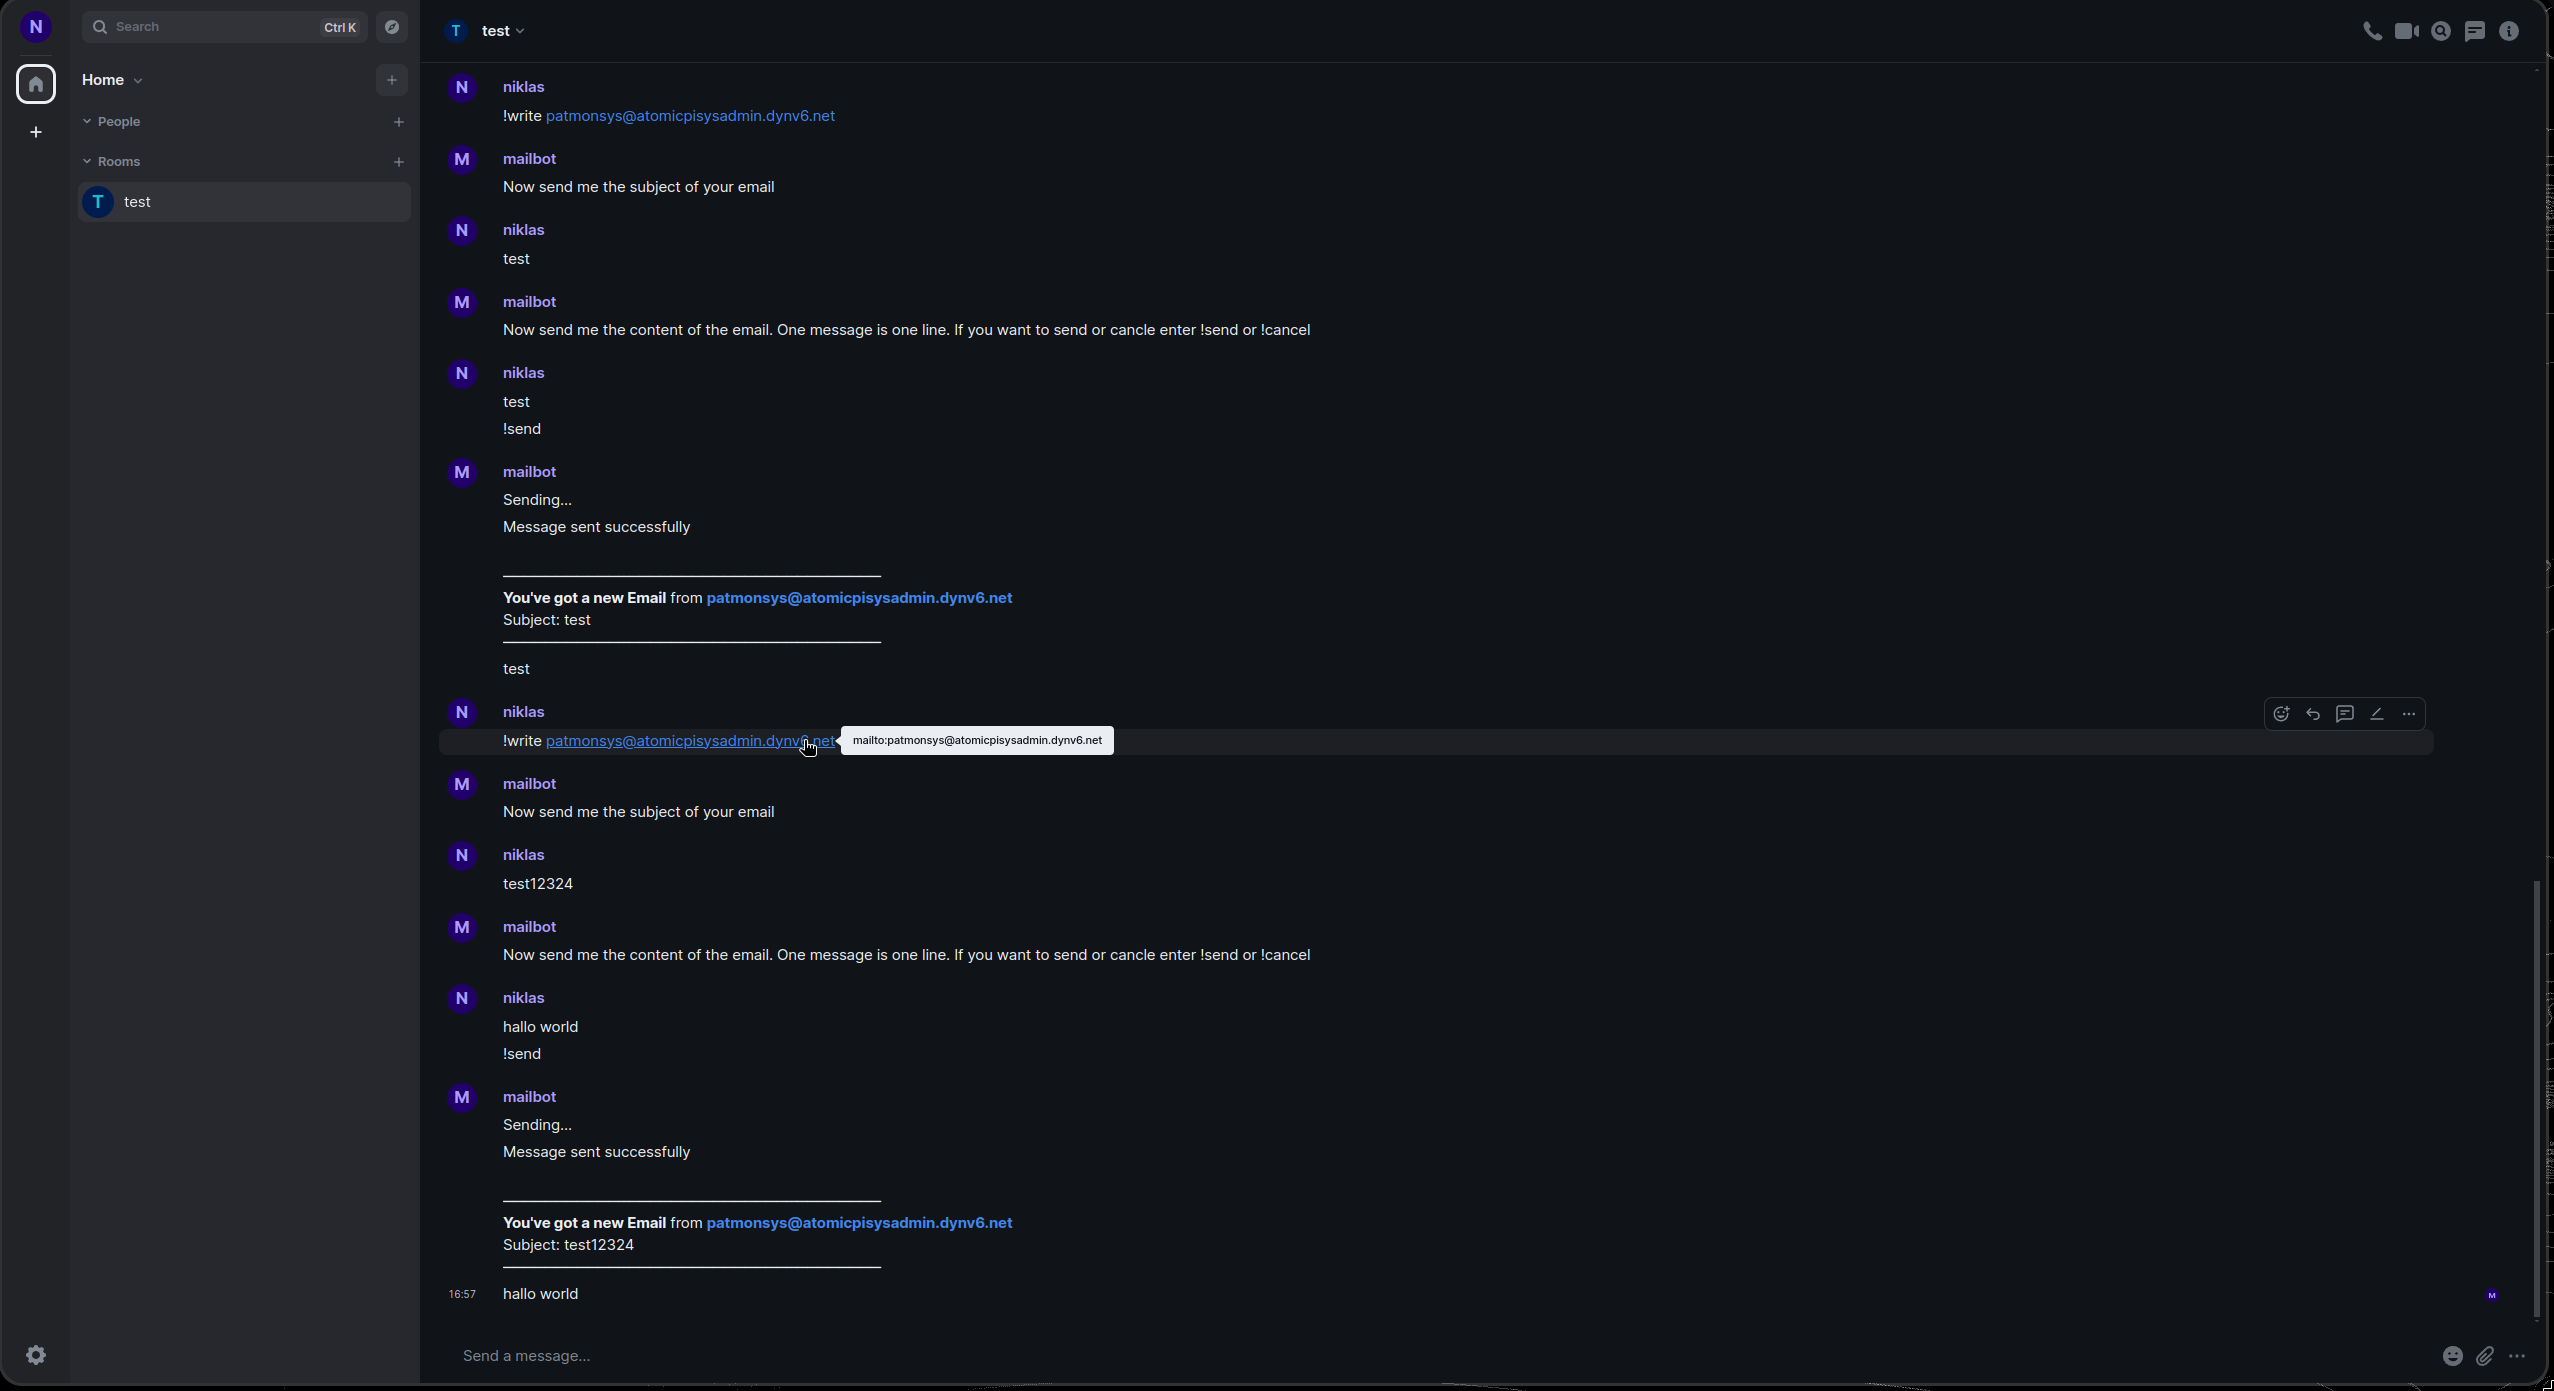
\includegraphics[width=\textwidth]{Images/Matrix.png} 
		\caption*{E-Mail Bridge in Element}
	\end{minipage}
	\hfill
	\caption{Matrix Setup}
	\label{fig:Matrix}
\end{figure} 
\end{frame}


\section{Todo}
\begin{frame}
\frametitle{Todo}
\begin{enumerate}
    \item Zusammenführen der Systeme
    \item Evaluation
    \item Mailcow
    \item Alarm Setup
\end{enumerate}
\end{frame}


\end{document} 